\documentclass[12pt,a3paper]{article}
\usepackage[a3paper,margin=9mm]{geometry}
\usepackage[T1]{fontenc}
\usepackage[scaled]{helvet}
\usepackage{qrcode}
\renewcommand{\familydefault}{\sfdefault}
\usepackage{graphicx,amsmath,booktabs,array,xcolor,tcolorbox,enumitem,adjustbox,hyperref}
\tcbuselibrary{skins}
\pagestyle{empty}
\setlength{\parindent}{0pt}
\setlength{\parskip}{1.4pt}
\setlist[itemize]{leftmargin=4.6mm,itemsep=0.5pt,topsep=1pt,parsep=0pt}
\setlist[enumerate]{leftmargin=4.6mm,itemsep=0.5pt,topsep=1pt,parsep=0pt}
\definecolor{navy}{HTML}{1F3864}
\definecolor{blue}{HTML}{2E75B6}
\definecolor{ink}{HTML}{182A42}
\color{ink}
\hypersetup{colorlinks=true,urlcolor=blue}
\newtcolorbox{posterblock}[1]{enhanced,colback=white,colframe=blue,colbacktitle=blue,coltitle=white,fonttitle=\bfseries\large,title={#1},boxrule=0.8pt,arc=2mm,top=1.5mm,bottom=1.5mm,left=2.5mm,right=2.5mm,toptitle=1.1mm,bottomtitle=1.1mm,before skip=0mm,after skip=1.5mm}
\newcommand{\figcap}[1]{{\footnotesize\color{navy}\itshape #1\par}}
\begin{document}
% ==================== TITLE: BITS TEMPLATE STYLE =====================
\noindent\begin{tcolorbox}[enhanced,colback=navy,colframe=navy,boxrule=0pt,arc=0mm,left=4mm,right=4mm,top=3mm,bottom=3mm]
\begin{minipage}[c]{0.17\linewidth}\centering

\includegraphics[width=0.84\linewidth,height=32mm,keepaspectratio]{bits_logo.png}
\end{minipage}%
\hfill%
\begin{minipage}[c]{0.80\linewidth}\centering\color{white}
{\bfseries\fontsize{21}{25}\selectfont Indoor Air Quality Anomaly Detection using LSTM Autoencoder\par}
\vspace{2mm}
{\fontsize{10.2}{13}\selectfont Nikhil Kumar Kambampati (2025H1400104P)\;\textbullet\; Akash Pasala (2025H1400043P)\par}
\vspace{1.2mm}
{\fontsize{9.4}{12}\selectfont Department of Electrical and Electronics Engineering, BITS Pilani, Pilani Campus\par}
{\fontsize{9.4}{12}\selectfont MLEE (EEE G513)\;\textbullet\; Instructor: Dr. Ritesh Vyas\par}
\end{minipage}
\end{tcolorbox}
\vspace{1.5mm}
% ===== SINGLE BOX FOR BOTH COLUMNS: prevents stacked minipages ======
\noindent\begin{adjustbox}{max totalsize={\textwidth}{0.86\textheight},center}
\begin{minipage}{\textwidth}
\fontsize{13.2}{15.5}\selectfont
\begin{minipage}[t]{0.485\linewidth}\vspace{0pt}
\begin{posterblock}{Summary}
Indoor air quality monitoring requires detection of unusual multivariate sensor patterns. We developed an unsupervised LSTM Autoencoder using DALTON kitchen recordings and compared it with Isolation Forest. On a \textbf{controlled synthetic evaluation}, LSTM achieved \textbf{96.80\% accuracy} and \textbf{96.90\% F1-score}, versus 64.53\% and 46.23\% for the baseline.
\end{posterblock}
\begin{posterblock}{Introduction and Objectives}
\textbf{Motivation:} Detecting unusual changes in particulate matter, humidity, CO$_2$ and gas-sensor readings without verified anomaly labels can support indoor environmental monitoring.
\textbf{Objectives:}
\begin{itemize}
\item Develop a temporal LSTM Autoencoder for 10 sensor measurements.
\item Compare it against an unsupervised Isolation Forest baseline.
\item Examine reconstruction errors, sensor changes, and activity annotations.
\end{itemize}
\end{posterblock}
\begin{posterblock}{Background}
\textbf{LSTM Autoencoder:} An encoder compresses a multivariate sequence; a decoder reconstructs it. High mean squared reconstruction error indicates unusual patterns:
\[\mathrm{MSE}=\frac{1}{TF}\sum_{t=1}^{T}\sum_{f=1}^{F}(x_{tf}-\hat x_{tf})^2,\quad T=60,\ F=10.\]
\textbf{Isolation Forest:} Isolates unusual observations through random partitions; it provides an efficient, unlabeled baseline [2].
\textbf{Gap:} Test whether temporal modeling improves sensitivity to injected sensor disturbances.
\end{posterblock}
\begin{posterblock}{Methodology}
\begin{center}
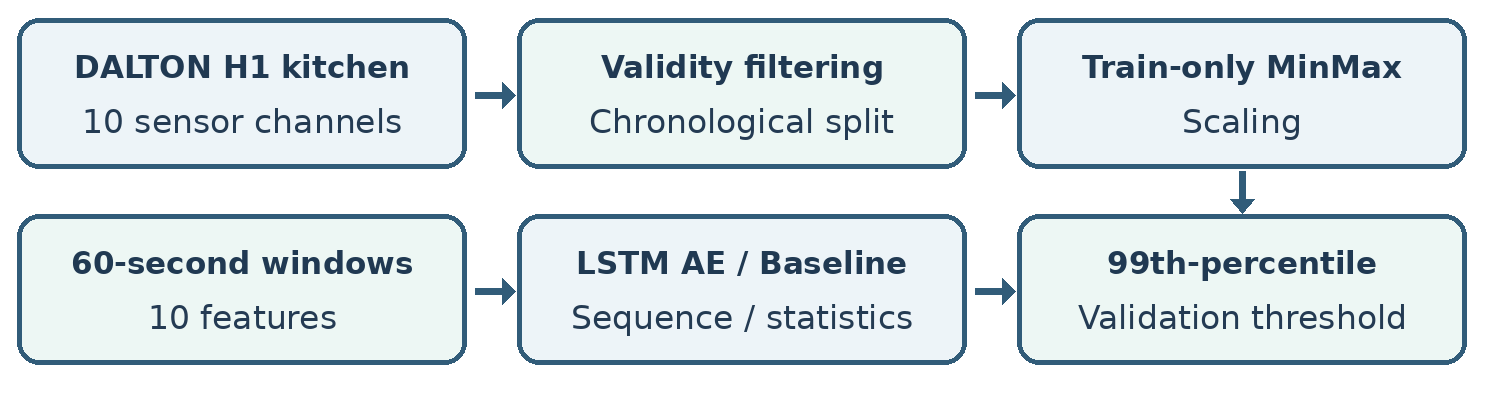
\includegraphics[width=0.96\linewidth,height=41mm,keepaspectratio]{fig_method.png}
\par\vspace{0.5mm}\figcap{Figure 1. Leakage-aware IAQ anomaly detection pipeline.}
\end{center}
\begin{enumerate}
\item \textbf{Preprocess:} Filter invalid/all-zero readings; preserve recording gaps.
\item \textbf{Normalize:} Fit MinMaxScaler only on training readings.
\item \textbf{Window:} Generate 60-second sequences of 10 features.
\item \textbf{Train:} LSTM Autoencoder and 40-feature Isolation Forest.
\item \textbf{Detect:} Apply each model's validation 99th-percentile threshold.
\end{enumerate}
\end{posterblock}
\begin{posterblock}{Experimental Setup}
\small\renewcommand{\arraystretch}{1.07}
\begin{tabular}{@{}p{0.34\linewidth}p{0.62\linewidth}@{}}
\toprule\textbf{Parameter}&\textbf{Configuration}\\\midrule
Dataset / site&DALTON, H1 Kitchen, sensor 41\\
Split (train / val / test)&48.7\% / 17.1\% / 34.2\% (by windows)\\
Chronological dates&May 28--30 / May 31 / Jun 4--5, 2023\\
Sequences (train / val / test)&246,009 / 86,282 / 172,564\\
LSTM architecture&32--16 bottleneck--32; 15,242 parameters\\
Training&30 epochs, batch 256, Adam, MSE\\
Isolation Forest&200 trees; 40 statistical features\\
Environment&Python, TensorFlow, scikit-learn, Colab T4\\
\bottomrule
\end{tabular}
\end{posterblock}
\end{minipage}%
\hfill%
\begin{minipage}[t]{0.485\linewidth}\vspace{0pt}
\begin{posterblock}{Results}
\textbf{A. Baseline comparison (synthetic evaluation)}
\begin{center}
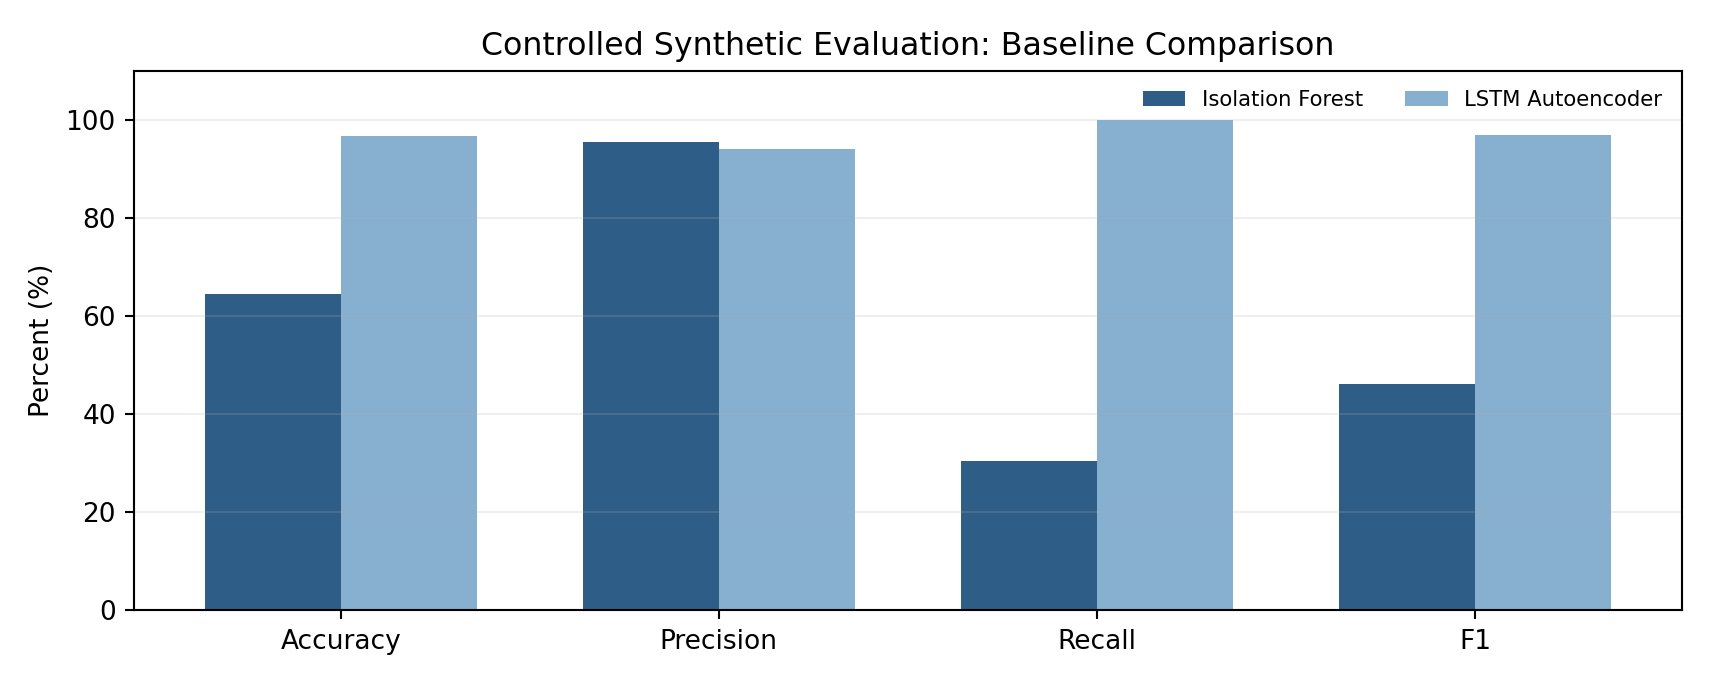
\includegraphics[width=0.96\linewidth,height=43mm,keepaspectratio]{fig_result1.png}
\par\vspace{0.5mm}\figcap{Figure 2. LSTM improves recall and F1-score on injected disturbances.}
\end{center}
\small\renewcommand{\arraystretch}{1.09}
\begin{center}
\begin{tabular}{@{}lrrrr@{}}
\toprule\textbf{Method}&\textbf{Acc.}&\textbf{Prec.}&\textbf{Rec.}&\textbf{F1}\\\midrule
Isolation Forest&64.53&\textbf{95.46}&30.50&46.23\\
\textbf{LSTM AE}&\textbf{96.80}&93.98&\textbf{100.00}&\textbf{96.90}\\
\bottomrule
\end{tabular}
\end{center}
\figcap{Table 1. Controlled synthetic evaluation (\%); not real-world accuracy.}
\vspace{1.3mm}
\textbf{B. Real-data anomaly and feature analysis}
\begin{center}
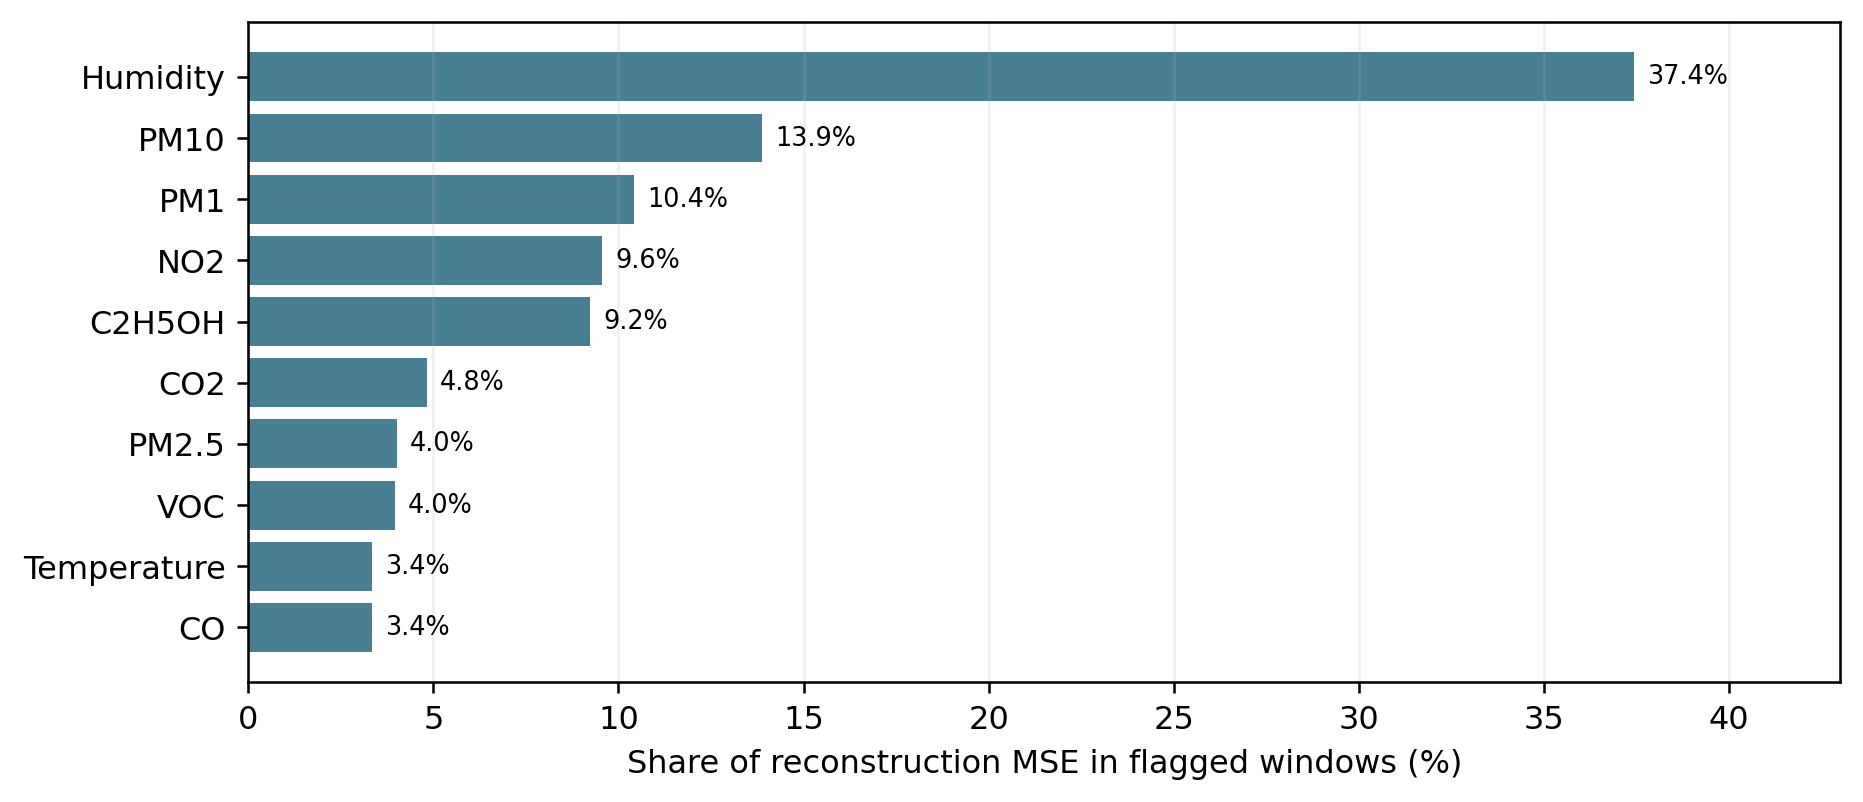
\includegraphics[width=0.96\linewidth,height=42mm,keepaspectratio]{fig_result2.png}
\par\vspace{0.5mm}\figcap{Figure 3. Feature-wise share of reconstruction MSE in flagged windows.}
\end{center}

\begin{itemize}
\item \textbf{Real DALTON test:}
172,564 windows across two unseen dates.

\item \textbf{LSTM Autoencoder:}
11,623 flagged windows (6.74\%).

\item \textbf{Isolation Forest:}
2,251 flagged windows (1.30\%).

\item \textbf{Event analysis:}
23 LSTM detection events; 27/165 activity
annotations had nearby flags ($\pm 5$ min).

\item \textbf{Feature analysis:}
Humidity contributed 37.42\% of
reconstruction MSE in flagged windows.
\end{itemize}

\end{posterblock}
\begin{posterblock}{Discussion}
\begin{itemize}
\item \textbf{Strength:} LSTM detected 2,000/2,000 synthetic disturbances; Isolation Forest detected 610/2,000.
\item \textbf{Trade-off:} LSTM flagged 128 unmodified test windows; Isolation Forest flagged 29 (assumed-normal labels).
\item \textbf{Event evidence:} Several high-error periods matched significant sensor shifts near cooking records.
\item \textbf{Limitation:} Activity annotations are not verified anomaly ground truth; synthetic perturbations were relatively strong.
\end{itemize}
\end{posterblock}
\begin{posterblock}{Conclusion and Future Work}
\begin{itemize}
\item LSTM synthetic F1 was \textbf{96.90\%} vs. \textbf{46.23\%} for the baseline.
\item Cooking-associated events provide plausible contextual evidence, not proof of causation.
\item \textbf{Next:} Verified anomaly labels; additional rooms/dates; weaker disturbance tests.
\end{itemize}
\end{posterblock}
\begin{minipage}[t]{0.64\linewidth}\vspace{0pt}
\begin{posterblock}{References}
\scriptsize
[1] P. Malhotra et al., ``LSTM-based Encoder-Decoder for Multi-sensor Anomaly Detection,'' arXiv:1607.00148, 2016.\par
[2] F. T. Liu, K. M. Ting, Z.-H. Zhou, ``Isolation Forest,'' IEEE ICDM, 2008.\par
[3] DALTON, \url{https://github.com/prasenjit52282/dalton-dataset}.
\end{posterblock}
\end{minipage}%
\hfill%
\begin{minipage}[t]{0.34\linewidth}\vspace{0pt}


% ============================================================
% REPORT AND CODE
% ============================================================

\begin{posterblock}{Report and Code}

\centering

% GitHub QR Code
\qrcode[height=16mm]{
https://github.com/Nikhilkumar-30/IAQ-Anomaly-Detection-LSTM-Autoencoder
}

\vspace{1.5mm}

{\scriptsize\bfseries
Scan for Report and Code
}

\vspace{2mm}

\raggedright
\scriptsize

\textbf{Contact:}\\
{
Nikhil: h20250104@pilani.bits-pilani.ac.in
}\par
{
Akash: h20250043@pilani.bits-pilani.ac.in
}

\vspace{2mm}

\textbf{Acknowledgements:}\\
We thank Dr. Ritesh Vyas for his guidance,
BITS Pilani for academic resources,
and the DALTON dataset contributors
for making the data available.

\end{posterblock}


\end{minipage}
\end{minipage}
\end{minipage}
\end{adjustbox}
\end{document}
